% !TeX program = lualatex

% Per https://github.com/matze/mthemem, Fira fonts needs to be installed in the system.
% If fonts do not metter, just use pdflatex instead of lualatex (and also remove luatex85 depnedency below)

\documentclass{beamer}
\usetheme{metropolis}

\usepackage{luatex85}
\usepackage{graphicx}
\usepackage{qrcode}

\usepackage{mathtools}
\mathtoolsset{showonlyrefs}

% https://stackoverflow.com/a/722954/2098471
\usepackage{chngpage}
\newenvironment{widecenter}{\begin{adjustwidth}{-1cm}{-1cm}\begin{center}}{\end{center}\end{adjustwidth}}

\usepackage[absolute,overlay]{textpos}
\setlength{\TPHorizModule}{\paperwidth}
\setlength{\TPVertModule}{\paperheight}

% https://tex.stackexchange.com/a/43005
\newlength{\currentparskip} 
\newenvironment{minipageparskip}[1]{\setlength{\currentparskip}{\parskip}\begin{minipage}{#1}\setlength{\parskip}{\currentparskip}}{\end{minipage}}

\usepackage{multimedia}
\setlength\unitlength{1cm}
\newcommand{\resvideo}[3]{\movie[width=#2cm,height=#3cm,poster,loop]{\framebox(#2,#3){\includegraphics[width=0.375cm]{res/video.png}\texttt{ #1{\footnotesize.mp4}}}}{video/#1.mp4}}

\usepackage{tikz}
\usetikzlibrary{arrows}
\usepackage{pgfplots}

% END OF CONFIGURATION

\title{MAE 259B Group 2 Final Presentation}
\date{06/06/2018}
\author{Siyuan Chen, Xiangzhou Kong, Long Chen}

\begin{document}
    \maketitle
    \begin{frame}{Background}
    	Elasticity and inner pressure of a ball is related to the rebounding motion of the ball.
    	\begin{center}
    		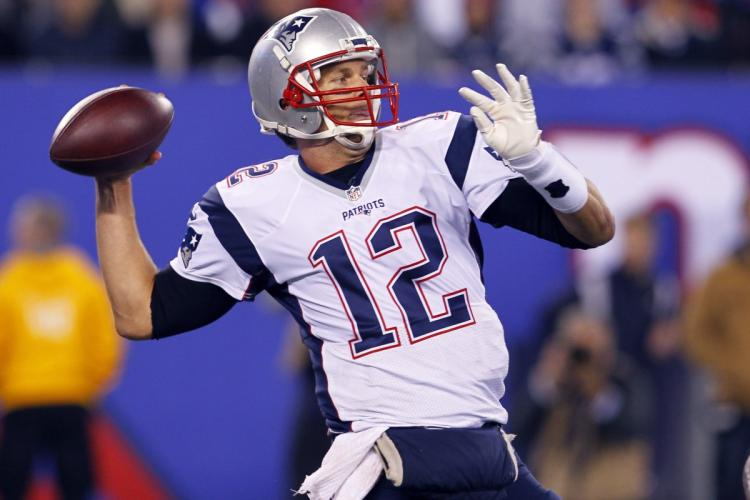
\includegraphics[width=0.5\textwidth]{res/football.jpg}\\
    		\footnotesize Deflegate scandal of New England Patriots
    	\end{center}
    \end{frame}
    \begin{frame}{Background}
    	\begin{center}
			\begin{tabular}{c|c}
				\textbf{Finite Element Method} & \textbf{Discrete Elastic Rod Model}\\
				& \\\hline
				& \\
				Widely used in industry & What we are doing in this project\\
				Abaqus, CATIA, ANSYS, etc. & (A lot faster)
			\end{tabular}
		\end{center}
	\end{frame}
    \begin{frame}{Review of our midterm presentation}
    	Started from simplest 2D DER
    	\begin{itemize}
    		\item Performance optimization (pre-computing reused terms)
    		\item Initial curvature
    		\item Circular structure
    		\item Inflation pressure (models as force-per-unit-length)
    		\item Surface contact (naïve predictor-corrector)
    		\item Damping (relative to center-of-mass)
    		\item Adaptive time stepping (limit momentum change per step)
    		\item Dynamic friction (partially Euler-forward)
    	\end{itemize}
    \end{frame}
	\begin{frame}{Review of our midterm presentation}
		\textbf{Bouncing ring structure on surface w/o and w/ friction}
		
		\begin{widecenter}
			\resvideo{no-friction}{6.856875}{5.214375}
			\resvideo{friction-0.2}{5.175}{5.214375}
		\end{widecenter}
		{\tiny Not all PDF viewers can play videos. Videos files can be alternatively found at \url{https://github.com/kmxz/mae259b/tree/master/final-presentation/video}}.
	\end{frame}
	\begin{frame}{Review of our midterm presentation}
		\textbf{Damping}
		
		Naïve damping $\underline F_{d,i} \propto -\underline u_i$ ruins bulk motion (as our bulk velocity is high)
		
		Use velocity relative to center of mass: $\underline F_{d,i} \propto -(\underline u_i - \underline u_{cm})$
		\vspace{0.5cm}
		\begin{widecenter}
			\begin{tabular}{ccc}
				No damping & Naïve damping & CM-Relative damping \\
				\resvideo{no-damp}{3.8467}{3.11} & 
				\resvideo{bad-damp}{3.6467}{3.11} & 
				\resvideo{good-damp}{3.8467}{3.11}
			\end{tabular}	
		\end{widecenter}
	\end{frame}
	\begin{frame}{Review of our midterm presentation}
		\begin{minipageparskip}{0.45\textwidth}
			\small
			\textbf{Adaptive time stepping}
			
			After trying $\Delta x$, $\Delta v$ and contact as criteria for determining time step size, we resulted in using momentum change as the optimal criteria.
			
			Step size should be inverse proportional to the maximum nodal reaction force from the ground.\\
			We limit $(F_{max})(dt)$ to a threshold ($\approx 0.005\,\mathrm{N\cdot s}$) for momentum change per step.
		\end{minipageparskip}%
		\begin{minipageparskip}{0.55\textwidth}
			\tiny
			\hfill
			\begin{tikzpicture}
			\begin{axis}[width=6cm,height=4cm,xlabel={$t$ [$\mathrm s$]},ylabel={$F_{max}$ [$\mathrm N$]},xmax=0.1,xticklabel style={/pgf/number format/fixed}]
			\addplot[black] table [x=t, y=f, col sep=comma, mark=none] {res/f-vs-dt.csv};
			\end{axis}
			\end{tikzpicture}
			
			\hfill
			\begin{tikzpicture}
			\begin{axis}[width=6cm,height=4cm,xlabel={$t$ [$\mathrm s$]},ylabel={$dt$ [$\mathrm s$]},xmax=0.1,xticklabel style={/pgf/number format/fixed}]
			\addplot[black] table [x=t, y=dt, col sep=comma, mark=none] {res/f-vs-dt.csv};
			\end{axis}
			\end{tikzpicture}
		\end{minipageparskip}
	\end{frame}
	\begin{frame}{Review of our midterm presentation}
		Adaptive time stepping:
		
		\begin{widecenter}
			\resvideo{ats}{11.388}{5.076}
		\end{widecenter}
	\end{frame}
	\begin{frame}{After midterm presentation}
		We spent quite some time trying to write a 3-D discrete shell simulation in C++.
		
		But we gave up, considering the limited time and difficulty in debugging.
		
		We continued improving the 2-D DER model.
	\end{frame}
	\begin{frame}{Improving visualization tool}
		Let viewport track the ring:
		
		\begin{widecenter}
			\resvideo{vp-track}{7.95}{5.598}
		\end{widecenter}
	\end{frame}
	\begin{frame}{Baraff-Witkin mass modification}
		For surface contact, we used Baraff-Witkin mass modification method to replace our naïve predictor-corrector method.
		
		Why?
		\begin{itemize}
			\item Our previous implementation need to extract sub-matrices of different sizes in each time step. With mass modification method, implementation can be neater.
			\item Our previous implementation only handles horizontal surface. With mass modification method, sloped surface can be included.
		\end{itemize}
	\end{frame}
	\begin{frame}{Baraff-Witkin mass modification}
		\begin{itemize}
			\item Detect DOFs to be constrained, just as before.
			\item Compute ``imposed velocity change'' $\underline z$ for those DOFs to stay above contact surface.
			\item In time marching, use $v_i$ instead of $x_i$:
			$$\frac{\delta v_i}{\delta t} = \frac{x_i(t_{k+1}) - x_i(t_k)}{(dt)^2} - \frac{v_i(t_k)}{dt}$$
			\item Therefore, EOM becomes: $\Delta \underline v - (dt) \underline{\underline w}\,\underline F - \underline z = 0$ 
			\item Inversed mass matrix $\underline{\underline w}$ is composed by $2\times2$ component matrices $\underline{\underline w_i}$, which is $\frac1{m_i}\begin{bmatrix}1 & 0\\0 & 1\end{bmatrix}$ for unconstrained nodes, $\frac1{m_i}(\underline{\underline I} - \underline n\,\underline n^T)$ for nodes constrained in $\underline n$ direction.
		\end{itemize}
	\end{frame}
	\begin{frame}{Baraff-Witkin mass modification}
		\textbf{Newton-Raphson iteration}
		
		Since we are solving for $\Delta \underline v$, in each iteration:
		$$\Delta \underline v \gets \Delta \underline v - \underline{\underline J} \textbackslash \underline f$$
		
		where $\underline f = \Delta \underline v - (dt)\underline{\underline w}\,\underline F - z$ and $\underbrace{\underline{\underline J}}_{\frac{\partial \underline F}{\partial \Delta \underline v}} = \underline{\underline I} - (dt)^2\underbrace{\underline{\underline J}^{old}}_{\frac{\partial \underline F}{\partial \underline x}}$
	\end{frame}
	\begin{frame}{Baraff-Witkin mass modification}
		Yeah, sloped surface.
		\begin{widecenter}
			\resvideo{sloped}{10.9714}{5.3314}
		\end{widecenter}
	\end{frame}
	\begin{frame}{Baraff-Witkin mass modification}
		Yeah, sloped surface.
		\begin{widecenter}
			\resvideo{sloped-track}{8.3733}{6.22}
		\end{widecenter}
	\end{frame}
	\begin{frame}{Baraff-Witkin mass modification}
		The procedure of handling \textbf{non-zero friction}, as covered in class, is:
		
		\begin{enumerate}
			\item Constrain both directions ($x$, $y$) of a node (to emulate static friction)
			\item Decompose reaction force $\underline f_i$ into normal force $\underline f_i^{normal}$ and $\underline f_i^{friction}$ (by $\underline f^{normal} = \underline f_i\cdot\underline n_{wall}$ and $\underline f^{friction} = \underline f_i - \underline f_i^{normal}$)
			\item Test if $f_i^{friction} > \mu_{static} f_i^{normal}$. If so, release $x$-constraint and apply dynamic friction $\mu_{dynamic}f_i^{normal}$ instead. 
		\end{enumerate}
	
		However, in our scenario, normal force is always relatively small. $f_i^{friction} > \mu_{static} f_i^{normal}$ happens all the time. Static friction never get applied. Dynamic pressure is simply added to $F^{external}$.
	\end{frame}
	\begin{frame}{``Rolling ribbon'' (no internal ``pressure'')}
		Different Young's modulus, other parameters kept the same:
		\begin{widecenter}
			\resvideo{roll-2e6}{5.35875}{3.49875}
			\resvideo{roll-3e6}{5.35875}{3.49875}\\
			\resvideo{roll-4e6}{5.35875}{3.49875}
			\resvideo{roll-8e6}{5.35875}{3.49875}
		\end{widecenter}
	\end{frame}
	\begin{frame}{``Rolling ribbon'' (no internal ``pressure'')}
		\begin{widecenter}
			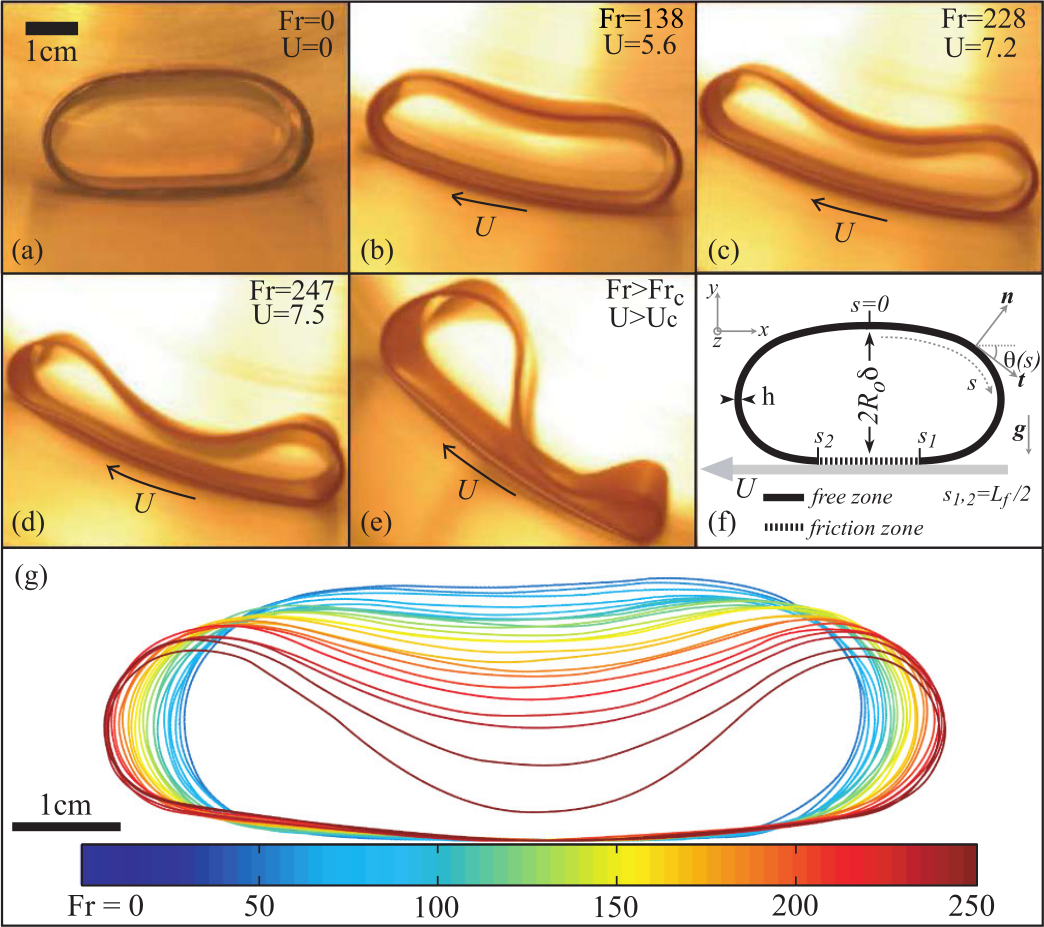
\includegraphics[width=0.5\textwidth]{res/rolling-ribbon.png}
			\hspace{0.25cm}
			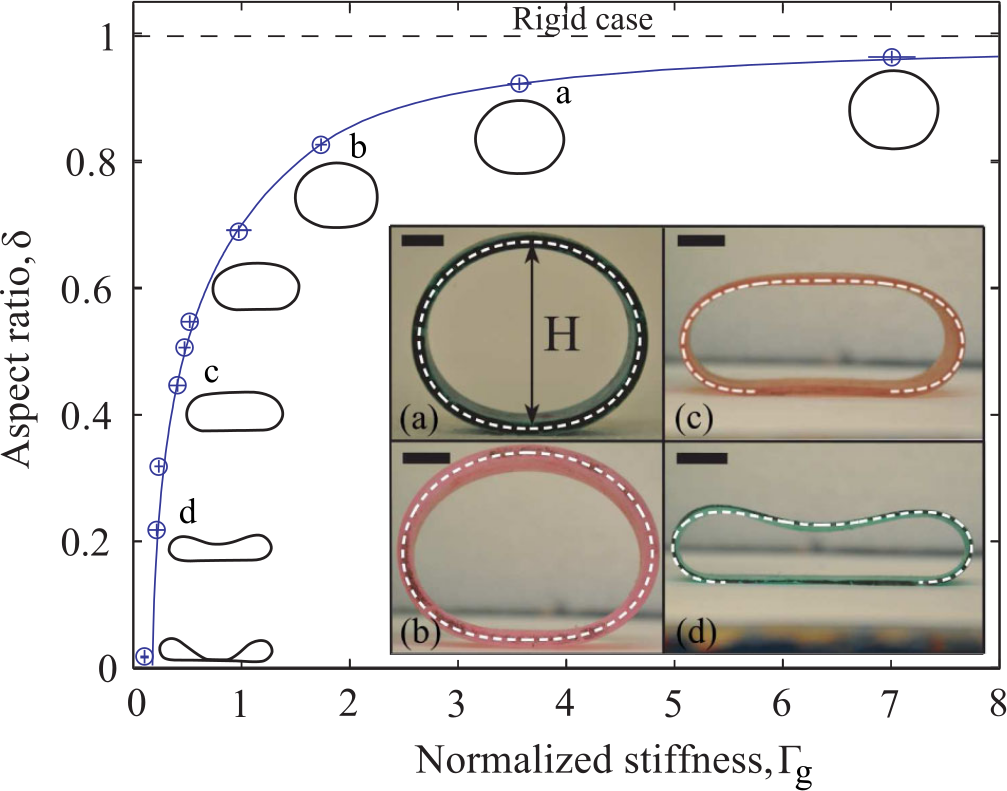
\includegraphics[width=0.525\textwidth]{res/ribbon.png}\\
			\footnotesize Figures from ``Rolling Ribbons'' (P. S. Raux \textit{et al.}, 2010)
		\end{widecenter}
	\end{frame}
	\begin{frame}{Variable inflation pressure}
		Recall that we discretized the inflation pressure as below:
		\begin{widecenter}
			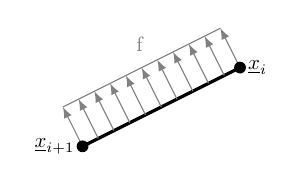
\begin{tikzpicture}[scale=0.5, every node/.style={scale=0.75}]
				\draw [very thick] (0,0) node [right] {$\underline x_i$} -- (-4,-2) node [left] {$\underline x_{i+1}$};
				\foreach \x in {0,...,10}
				\draw[gray,-latex,thin] (\x / 2.5 - 4,\x / 5 - 2) -- (\x / 2.5 - 4 - 0.5,\x / 5 - 2 + 1);
				\draw [gray,thin] (0 / 2.5 - 4 - 0.5,0 / 5 - 2 + 1) -- (10 / 2.5 - 4 - 0.5,10 / 5 - 2 + 1);
				\node [gray] at (5.5 / 2.5 - 4 - 0.75,5.5 / 5 - 2 + 1.5) {f};
				\node [circle,fill,minimum size=2mm,inner sep=0pt] at (0,0) {};
				\node [circle,fill,minimum size=2mm,inner sep=0pt] at (-4,-2) {};
			\end{tikzpicture}
			\hspace{0.1cm}
			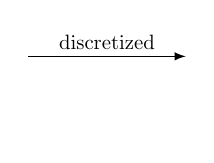
\begin{tikzpicture}[baseline=-1cm, every node/.style={scale=0.75}]
				\draw [-latex] (0,0) -- (2,0);
				\node [above] at (1,0) {discretized};
			\end{tikzpicture}
			\hspace{0.1cm}
			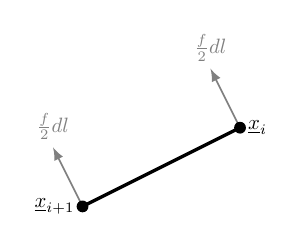
\begin{tikzpicture}[scale=0.5, every node/.style={scale=0.75}]
				\draw [very thick] (0,0) node [right] {$\underline x_i$} -- (-4,-2) node [left] {$\underline x_{i+1}$};
				\draw [gray,-latex,semithick] (0 / 2.5 - 4,0 / 5 - 2) -- (0 / 2.5 - 4 - 0.75,0 / 5 - 2 + 1.5) node [above] {$\frac{f}2 dl$};
				\draw [gray,-latex,semithick] (10 / 2.5 - 4,10 / 5 - 2) -- (10 / 2.5 - 4 - 0.75,10 / 5 - 2 + 1.5) node [above] {$\frac{f}2 dl$};
				\node [circle,fill,minimum size=2mm,inner sep=0pt] at (0,0) {};
				\node [circle,fill,minimum size=2mm,inner sep=0pt] at (-4,-2) {};
			\end{tikzpicture}
		\end{widecenter}
	
		However, instead of constant $f$, we may expect the pressure to get higher when the volume inside the structure is reduced. 
		
		For ideal gas:
		$$pV = nRT$$
		
		Assume the temperature is constant. Then $p \propto \frac1V$.
	\end{frame}
	\begin{frame}{Variable inflation pressure}
		For computing the internal volume, we take the area of the 2D ring. Since we already discretized the structure into a polygon, we can use shoelace formula to calculate area:
		$$A = \frac12\left[\sum_{i=1}^{n-1}x_iy_{i+1} + x_ny_1 - \sum_{i=1}^{n-1} x_{i+1}y_i - x_1y_n\right]$$
		
		Then, for each time frame, $p(t_k) = \frac{A(t_0)}{A(t_{k})}p(t_0)$
		
		We simple ignore this effects' contribution to Jacobian (otherwise the Jacobian will no longer be banded), it turns out we can still get convergence. 
	\end{frame}
	\begin{frame}{Variable inflation pressure}
		Variable inflation pressure does make results more realistic!
		
		\begin{widecenter}
			\resvideo{pressure-inv}{5.53}{4.665}
			\resvideo{pressure-var}{5.53}{4.665}
		\end{widecenter}
	\end{frame}
	\begin{frame}{Future improvements}
		\begin{itemize}
			\item 3-D shell (we've started, but shelved)
			\item Collision detection (we've started it, attempted for 2 different methods, but no good results achieved)
		\end{itemize}
	\end{frame}
\end{document}